%% -------------------
% Chih, Chao-Hsien
% Ver.1 20220219

\documentclass[a4paper]{article}

% Property of this paper
\newcommand{\className}{Control}
\newcommand{\classTeacher}{Prof.~ (~教授)}
\newcommand{\classPaperTitle}{Homework \#}



% ----------------------------------------------常用packege
\usepackage{latexsym}
\usepackage{amsmath,amssymb}
\usepackage{mathtools}
\usepackage[x11names]{xcolor}
\usepackage{graphicx}
\usepackage{algorithm}
\usepackage{amsthm}
\usepackage{lmodern} % 解決 font warning
\usepackage{animate} % insert gif

\usepackage{lipsum} % To generate test text 
\usepackage{ulem} % 下劃線,波浪線

\usepackage{listings} % display code on slides; don't forget [fragile] option after \begin{frame}
% ----------------------------------------------
% \usepackage[left=2.5cm, right=2.5cm, top=1.5cm, bottom=2.5cm]{geometry}
\usepackage{float}
% \usepackage{subfigure}
\usepackage{caption}
\usepackage{array}
\usepackage{bm}
\newcommand{\bmrm}[1]{\bm{\mathrm{#1}}}
\usepackage{algorithmicx}
\usepackage{algpseudocode}
\usepackage{hyperref}
\usepackage{animate}
\usepackage{movie15}
\usepackage{textcomp}
\usepackage{cite}
\usepackage{subfig}
\usepackage{makecell}
\usepackage{kantlipsum}% dummy text
\usepackage{stfloats}

% 縮排
\usepackage{indentfirst} 
\setlength{\parindent}{2em}

% 行距
\linespread{1.4}\selectfont

% xeCJK
\usepackage{xeCJK}
% 中文字體設定
\usepackage{fontspec} % 加這個就可以設定字體。
%設定中文為系統上的字型,而英文不去更動,使用原TEX字型。
\setCJKmainfont{ch}[
    Path=./Font/,
    UprightFont=KAIU.TTF,
    AutoFakeBold=3.0,
    AutoFakeSlant=0.0
    ]
\XeTeXlinebreaklocale "zh" %這兩行一定要加,中文才能自動換行。
\XeTeXlinebreakskip = 0pt plus 1pt % 這兩行一定要加,中文才能自動換行。

\setmainfont{Times New Roman}

% figure 設定
% ------ figure 路徑 ------
\graphicspath{{figure}} 
% ------ figure tag ------
\newcommand{\figuretag}[1]{%
    \addtocounter{figure}{-1}%
    \renewcommand{\thefigure}{#1}%
}
\captionsetup[figure]{labelfont={bf},name={Figure.},labelsep=period}
% ------ table tag ------
\newcommand{\tabletag}[1]{%
    \addtocounter{table}{-1}%
    \renewcommand{\thetable}{#1}%
}
\captionsetup[table]{labelfont={bf},name={Table.},labelsep=period}

% Uncomment and use as if needed
%\newtheorem{theorem}{Theorem}
% \newtheorem{lemma}[theorem]{Lemma}
\newdefinition{rmk}{Remark}
%\newproof{pf}{Proof}
%\newproof{pot}{Proof of Theorem \ref{thm}}




% 顯示程式碼設定
\usepackage{listings} % display code on slides; don't forget [fragile] option after \begin{frame}    
    \lstset{inputpath={code}}

    \definecolor{CcodeBlue}{rgb}{0,0,1}
    \definecolor{CcodeGreen}{rgb}{0,0.5,0}
    \definecolor{CcodeRed}{rgb}{0.64,0.08,0.08}

    \lstdefinestyle{C++}{
        language=C++,
        captionpos=b,                       % 讓Caption在Bottom的位置
        numbers=left,                       % 程式碼行號
        frame=lines,                        %開始結束有條黑線
        showstringspaces=false,             % "不"標註空格
        escapeinside={(@}{@)},            % 脫逃字元
        commentstyle=\color{CcodeGreen},         % Comment顏色
        keywordstyle=\color{CcodeBlue},          % Keyword顏色
        stringstyle=\color{CcodeRed},            % String顏色
        basicstyle=\ttfamily\small,         % 字型
  }

\definecolor{MatlabGreen}{RGB}{28,172,0} % color values Red, Green, Blue
\definecolor{MatlabLilas}{RGB}{170,55,241}

\lstdefinestyle{Matlab}{language=Matlab,%
    %basicstyle=\color{red},
    basicstyle=\ttfamily\small,         % 字型
    frame=lines,                        %開始結束有條黑線
    morekeywords={matlab2tikz},
    keywordstyle=\color{blue},
    morekeywords=[2]{1}, keywordstyle=[2]{\color{black}},
    identifierstyle=\color{black},
    stringstyle=\color{MatlabLilas},
    commentstyle=\color{MatlabGreen},
    showstringspaces=false,             %without this there will be a symbol in the places where there is a space
    numbers=left,%
    numberstyle={\tiny \color{black}},  % size of the numbers
    numbersep=9pt,                      % this defines how far the numbers are from the text
    emph=[1]{for,end,break},emphstyle=[1]\color{red}, %some words to emphasise
    %emph=[2]{word1,word2}, emphstyle=[2]{style},    
}

%% Matlab code block example 
% \begin{lstinputlisting}[style=Matlab]{main.m}
% \end{lstinputlisting}

%% C++ code block example
% \begin{lstlisting}[style=C++]
%   #include <iostream>
%   int main()
%   {
%       // Print Hello (@Test escapeinside@)
%       std::cout << "Hello, world!" << std::endl;
%       return 0;
%   }
% \end{lstlisting}


\newcommand{\ui}{u_{1}}
\newcommand{\suii}{s_{u_{2}}}
\newcommand{\cuii}{c_{u_{2}}}
\newcommand{\suiii}{s_{u_{3}}}
\newcommand{\cuiii}{c_{u_{3}}}
\newcommand{\sphi}{s_{\phi}}
\newcommand{\cphi}{c_{\phi}}
\newcommand{\stheta}{s_{\theta}}
\newcommand{\ctheta}{c_{\theta}}
\newcommand{\spsi}{s_{\psi}}
\newcommand{\cpsi}{c_{\psi}}
\newcommand{\sgn}{\mathrm{sgn}}

\title{Title}
\author{Name}
\date{\today}

\begin{document}

\begin{titlepage}
    \vspace*{1cm}
    \makeatletter
    \renewcommand{\thefootnote}{\@fnsymbol\c@footnote}
    \makeatother
    \setlength{\parindent}{0pt}
    \vspace{\baselineskip}

    {\LARGE \textsc{National Cheng Kung University}\par}
    {\Large Department of Aeronautics and Astronautics \\ Tainan, Taiwan, R.O.C.\par}

    \vspace{15em}

    {\Large {\classPaperTitle} \\ \className \par}

    \vspace{5em}

    \hfill\parbox{.9\linewidth}{%
        {
            \fontsize{12pt}{16pt}\selectfont
            \begin{tabular}{ll}
                % Instructor Name
                \textsc{\Large Instructor}: & {\classTeacher}\\
                % Student Name
                \textsc{\Large Student:} & {Chih, Chao-Hcien (池昭賢)}\\
                % Student ID
                \textsc{\Large Student ID:} & P46104269
            \end{tabular}
            }\par
    }\par
    \vspace{1em}
    \vspace{4\baselineskip}
    \today\par


\end{titlepage}


% \newpage
% \tableofcontents
% \addcontentsline{toc}{section}{Contents}
% \newpage
% \listoffigures
% \addcontentsline{toc}{chapter}{List of Figures}
% \newpage
% \listoftables
% \addcontentsline{toc}{chapter}{List of Tables}

% \newpage

這是一個模板供使用。

I'm writing to demonstrate use of automatically-generated footnote markers\footnote{Automatically generated footnote markers work fine!} and footnotes which use a marker value provided to the command
\footnote[42]{...is that the answer to everything?}.

Now, I will use another automatically-generated footnote marker
\footnote{Now, footnote markers are 1, 42, but then back to 2? That will be confusing if the automatically-generated number also reaches 42!}.

\section{Equation Example}


In this paper, the 3--2--1 intrinsic convention is considered. The direction cosine matrix (DCM), $\sideset{^\mathcal{G}}{^\mathcal{B}}{\mathop{\mathbf{C}}}(\phi, \theta, \psi)$, is constructed in terms of the Euler angles as follows:
\begin{equation} \label{eq::DCM}
    \sideset{^\mathcal{G}}{^\mathcal{B}}{\mathop{\mathbf{C}}}(\phi, \theta, \psi) = \mathbf{R}_z(\psi) \mathbf{R}_y(\theta)  \mathbf{R}_x(\phi)
\end{equation}
where
\begin{equation}
    \begin{aligned}
        \bmrm{R}_x(\phi) &=
        \begin{bmatrix}
            1 & 0      & 0     \\
            0 & \cphi  & -\sphi \\
            0 & \sphi & \cphi
        \end{bmatrix},\quad 
        \bmrm{R}_y(\theta) =
        \begin{bmatrix}
            \ctheta & 0 & \stheta \\
            0       & 1 & 0        \\
            -\stheta & 0 & \ctheta
        \end{bmatrix},\\
        \bmrm{R}_z(\psi) &=
        \begin{bmatrix}
            \cpsi  & -\spsi & 0 \\
            \spsi  & \cpsi & 0 \\
            0      & 0     & 1
        \end{bmatrix}
    \end{aligned}
\end{equation}
are the rotation matrices and the notations $s_{(\cdot)}$ and $c_{(\cdot)}$ represent $\sin(\cdot)$ and $\cos(\cdot)$, respectively. 

\begin{equation} \label{eq:attitude_error_dynamics}
    \begin{aligned}
        \dot{\bmrm{e}}_{1,\Theta} ={}& \bmrm{e}_{2,\Theta} \\
        \dot{\bmrm{e}}_{2,\Theta} ={}& -\bmrm{T}^{-1} \bmrm{J}^{-1} \bmrm{J}_0 \bmrm{T} \bigg(\bmrm{K}_{p,\Theta} \bmrm{e}_{1,\Theta} + \bmrm{K}_{i,\Theta} \int^t_0 \! \bmrm{e}_{1,\Theta}\,d\tau \\
        &+ \bmrm{K}_{d,\Theta} \bmrm{e}_{2,\Theta} \bigg) +\left[\bmrm{JT}\right]^{-1}\bmrm{d}_{\Theta} \\
        &+\left(\left[\bmrm{JT}\right]^{-1} \bmrm{J}_0 \bmrm{T} -\bmrm{I}_3 \right)\ddot{\bmrm{x}}_{1d,\Theta} \\
        &- \left[\bmrm{JT}\right]^{-1} \left( \left[ \bmrm{T}\bmrm{x}_{2,\Theta} \right]^{\times} \Delta \bmrm{J} \bmrm{T} \bmrm{x}_{2,\Theta} -\Delta \bmrm{J} \dot{\bmrm{T}}\bmrm{x}_{2,\Theta} \right)
    \end{aligned}
\end{equation}


\section{Figure Example}

\begin{figure}[H]
    \centering
    \subfloat[\label{fig:6Dof_Rocket_Dynamic_4}]{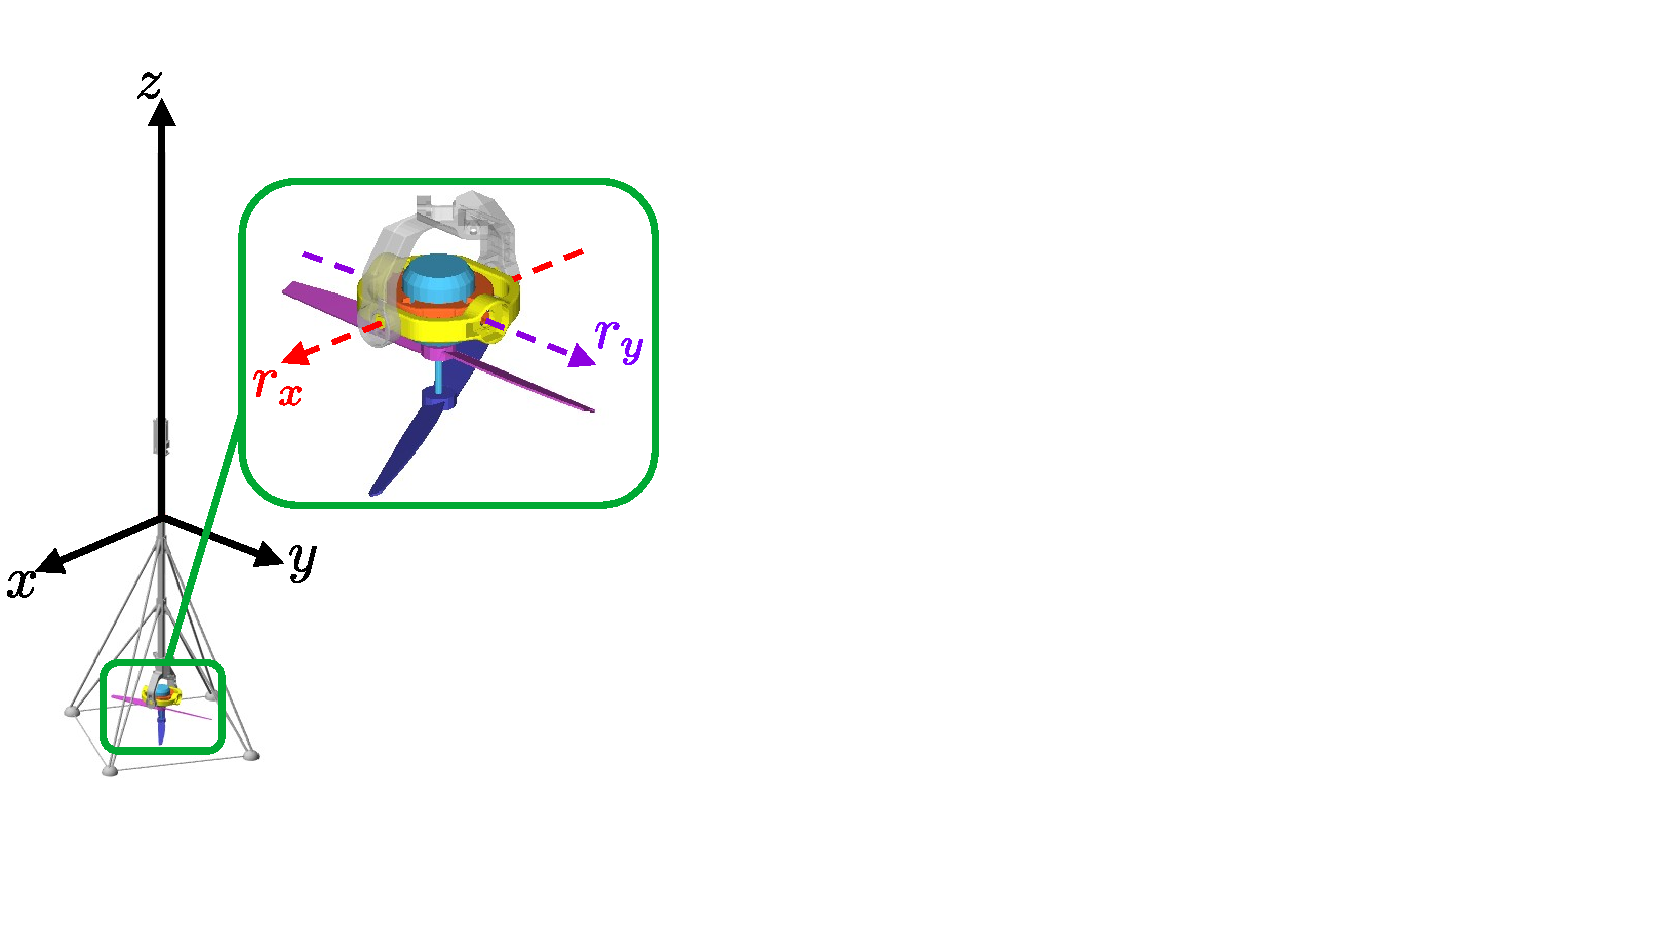
\includegraphics[width = 0.23\linewidth]{rdyyy_4.pdf}}
    \subfloat[\label{fig:6Dof_Rocket_Dynamic_1}]{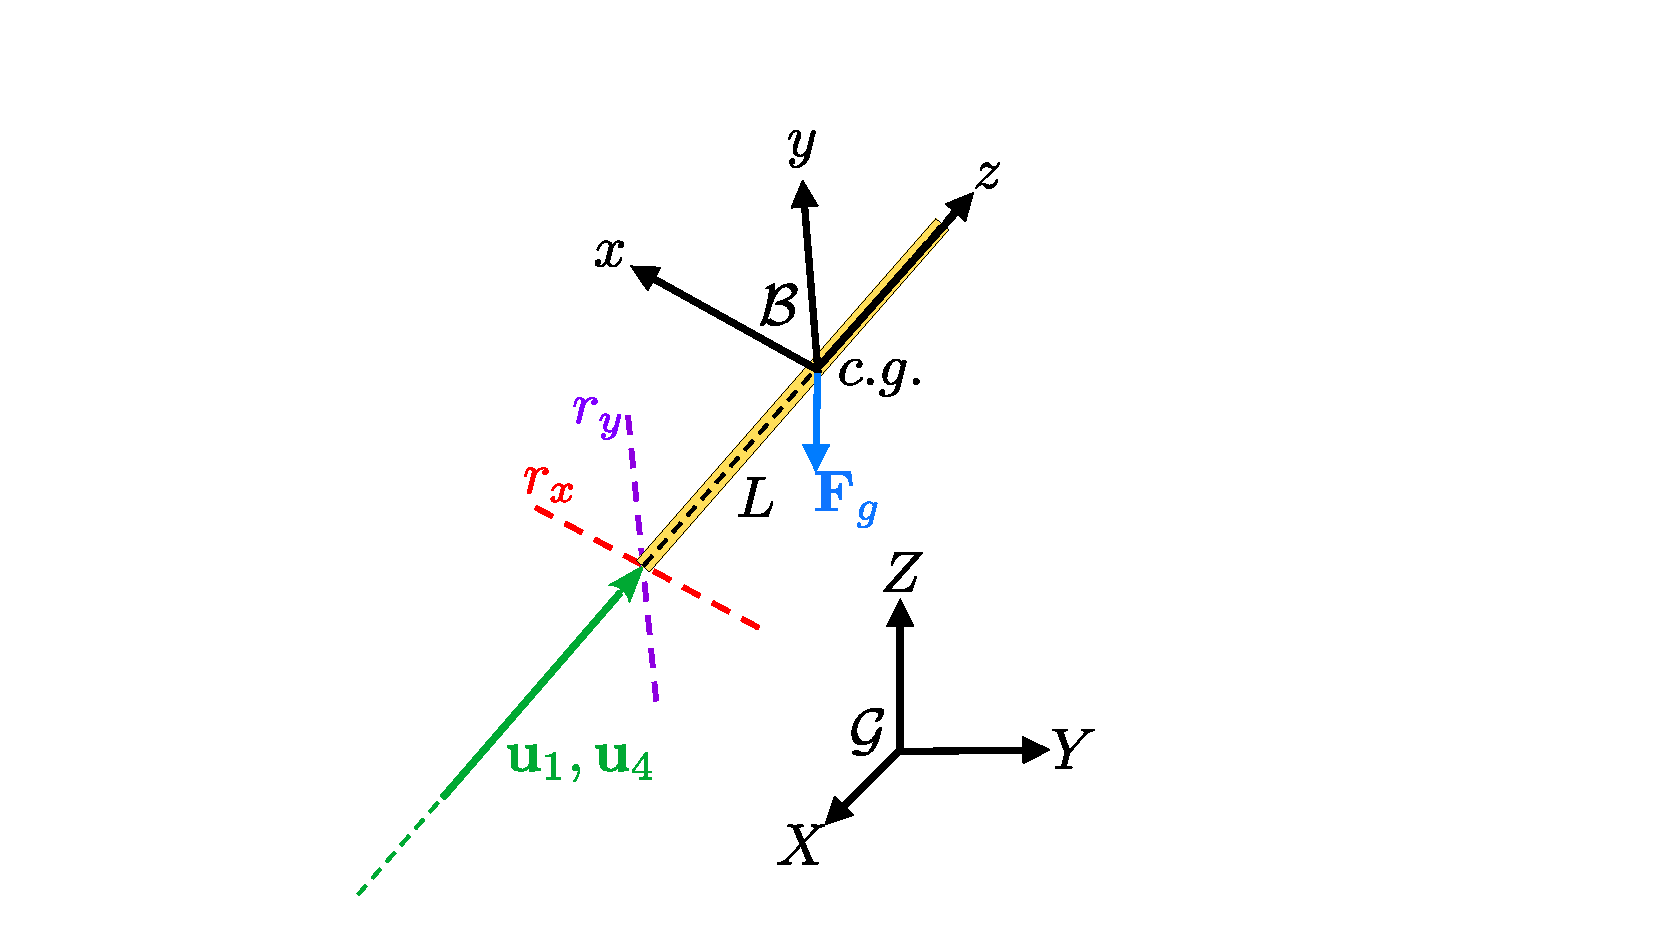
\includegraphics[width = 0.25\linewidth]{rdyyy_1.pdf}}\!
    \subfloat[\label{fig:6Dof_Rocket_Dynamic_2}]{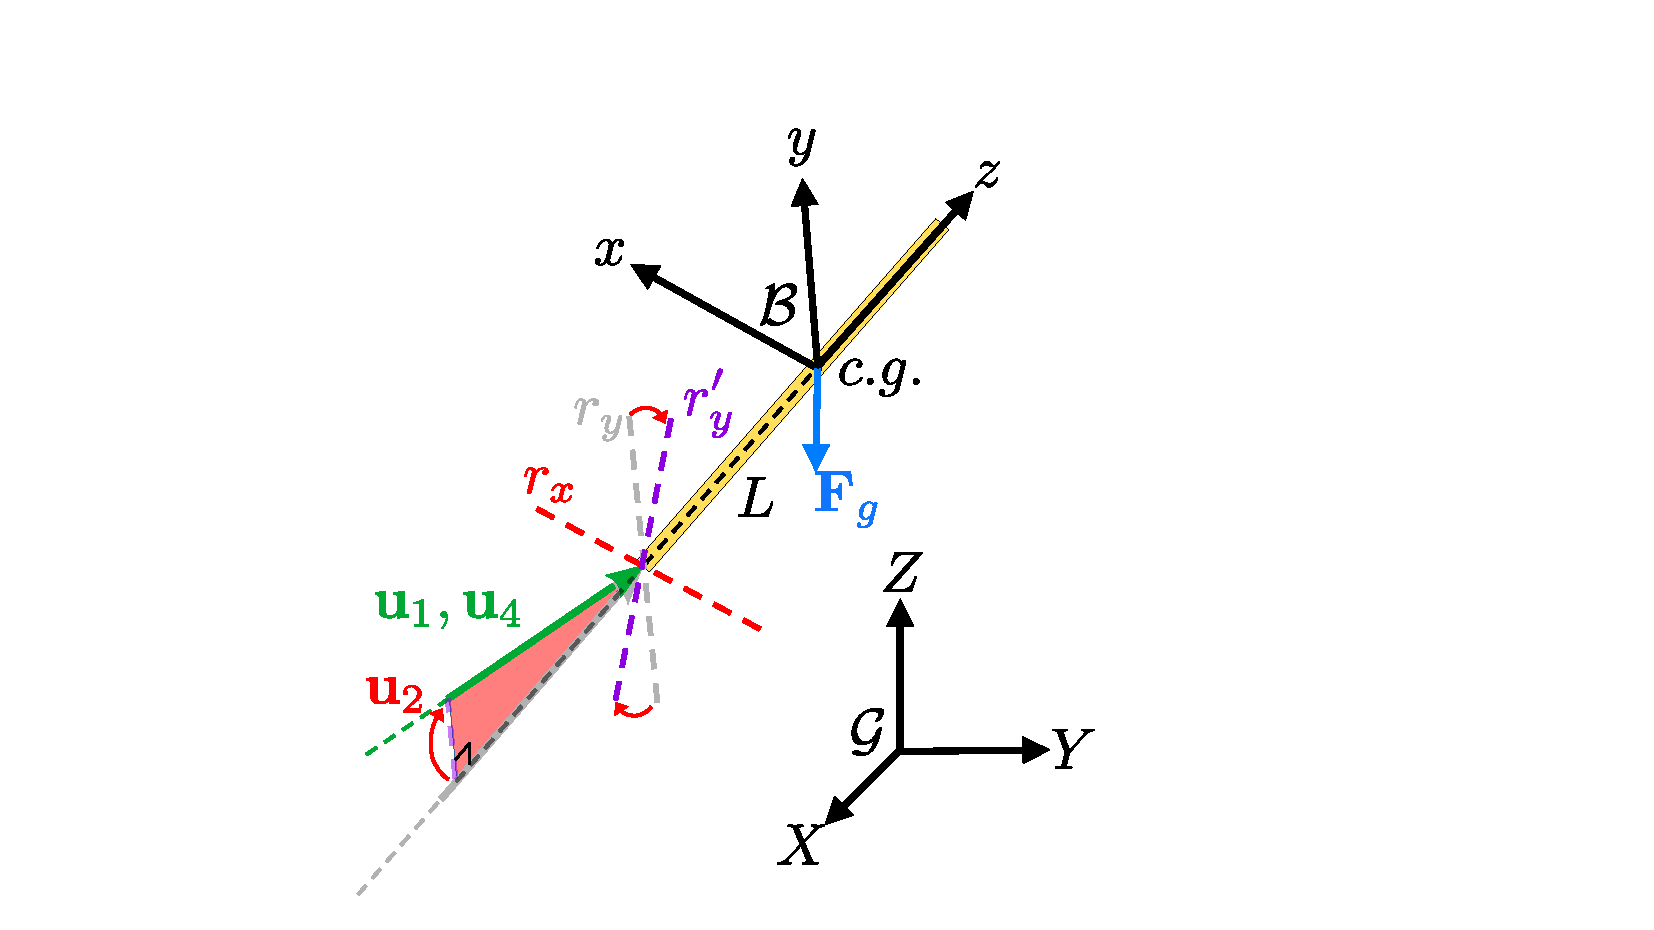
\includegraphics[width = 0.25\linewidth]{rdyyy_2.pdf}}\!
    \subfloat[\label{fig:6Dof_Rocket_Dynamic_3}]{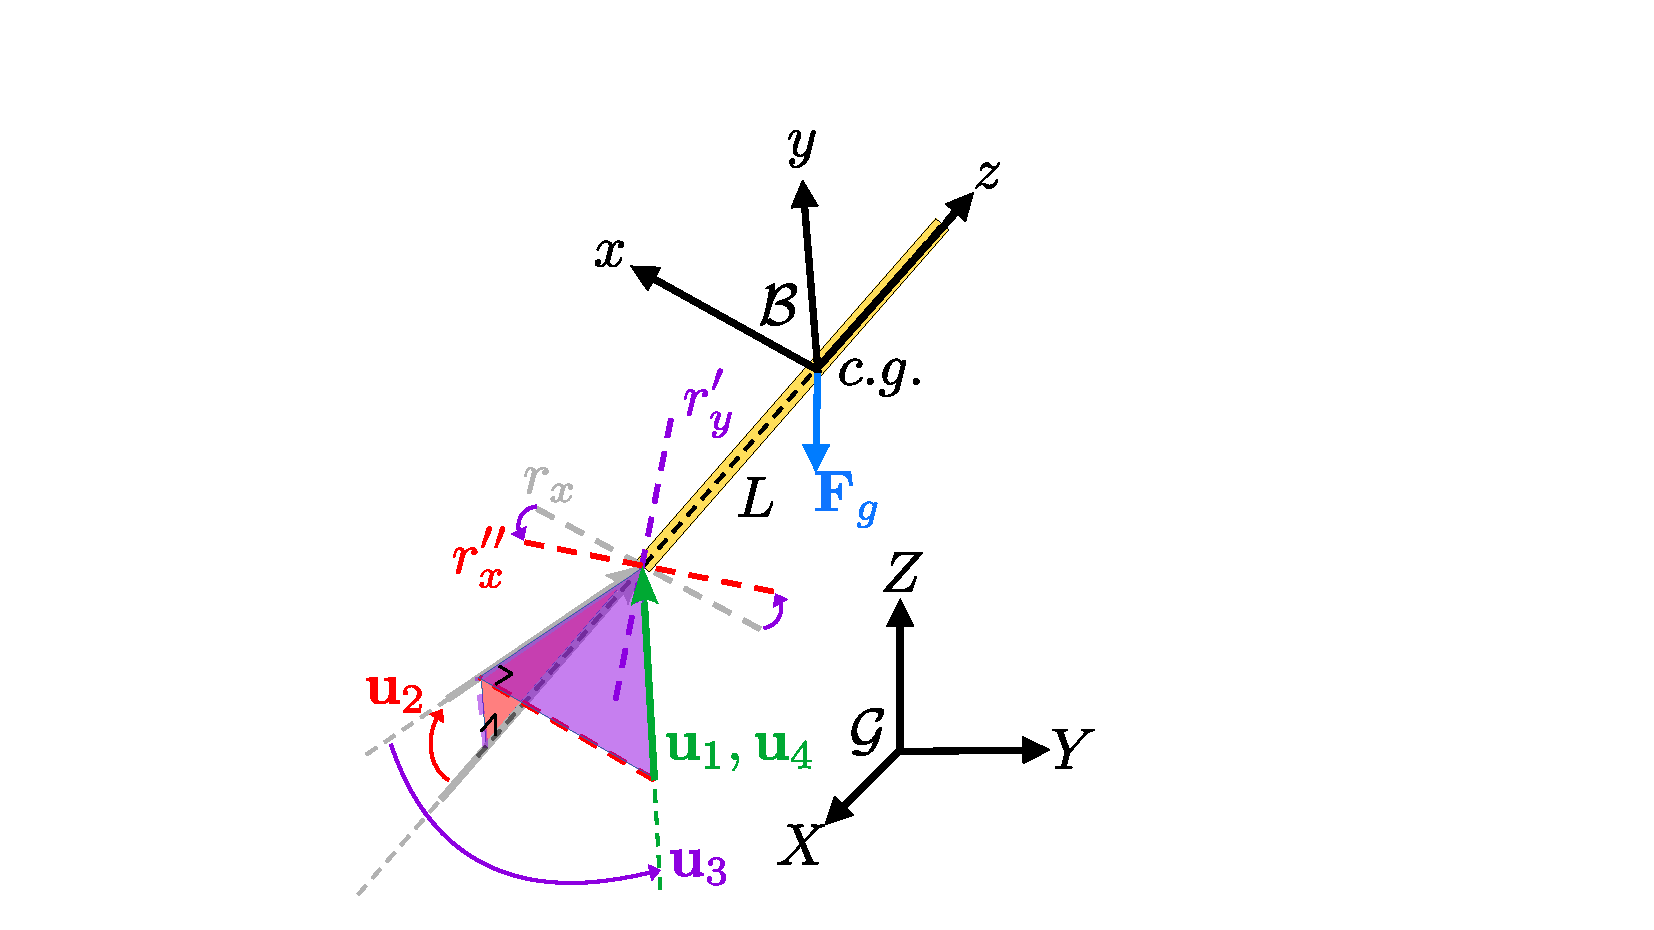
\includegraphics[width = 0.25\linewidth]{rdyyy_3.pdf}}
    \caption{Illustration of the rocket-type UAV force analysis.}
    \label{fig:6Dof_Rocket_Dynamics}
\end{figure}

\begin{figure}[H]
    \centering
    \begin{minipage}{0.3\linewidth}
        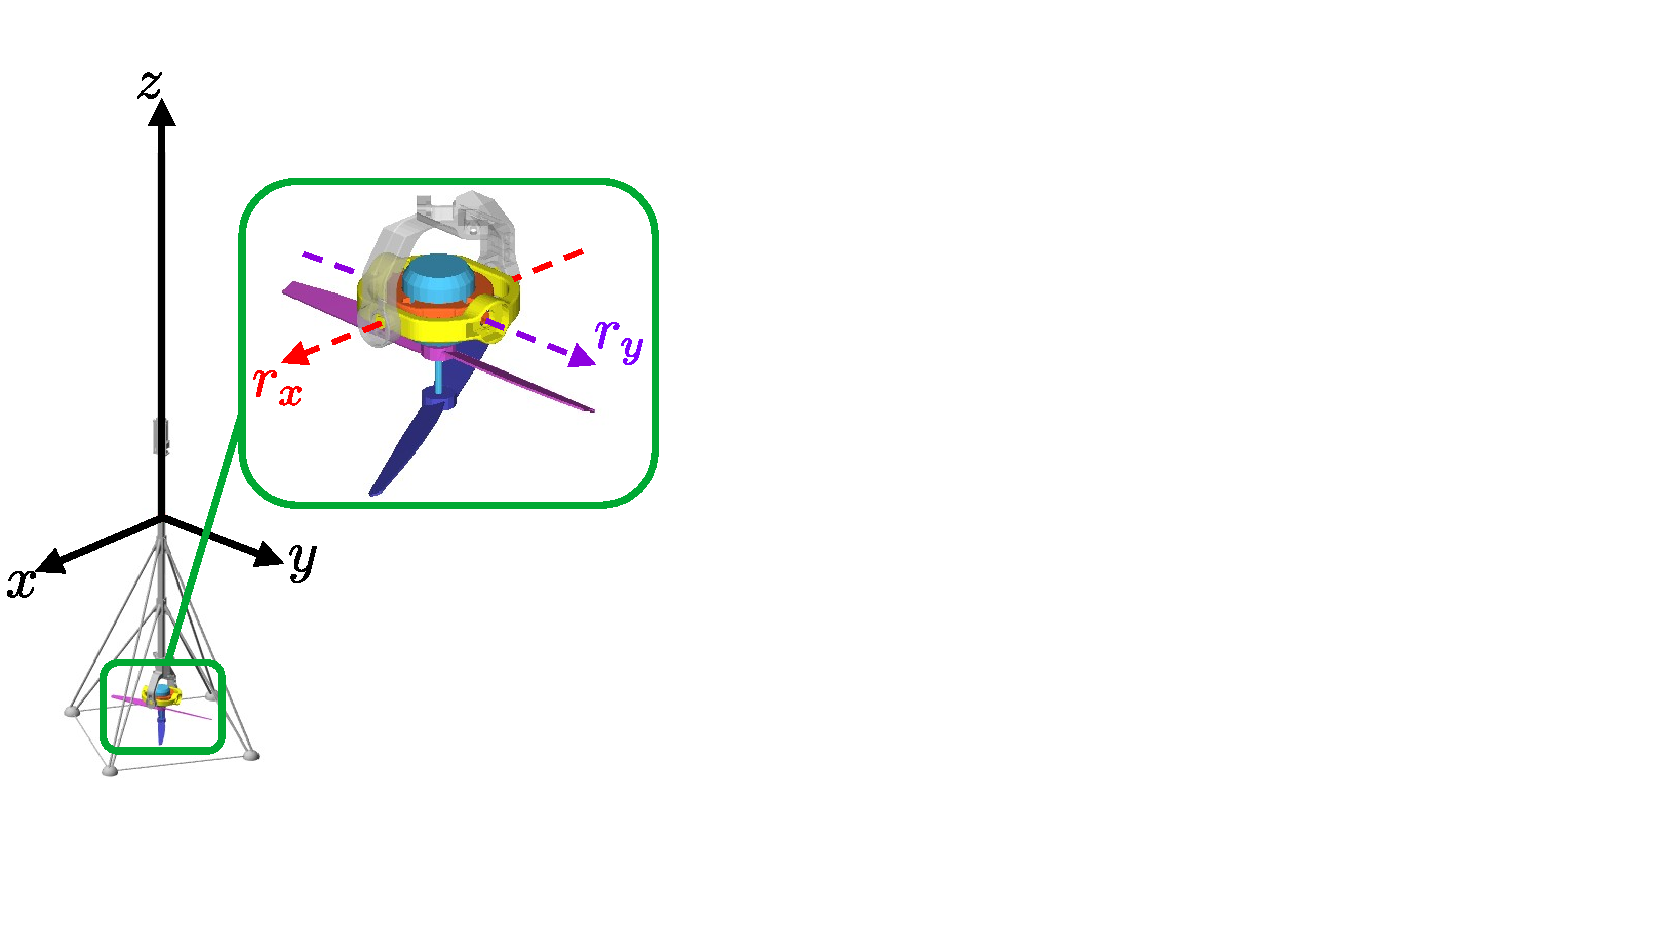
\includegraphics[width = \linewidth]{rdyyy_4.pdf}
    \end{minipage}
    \begin{minipage}{0.3\linewidth}
        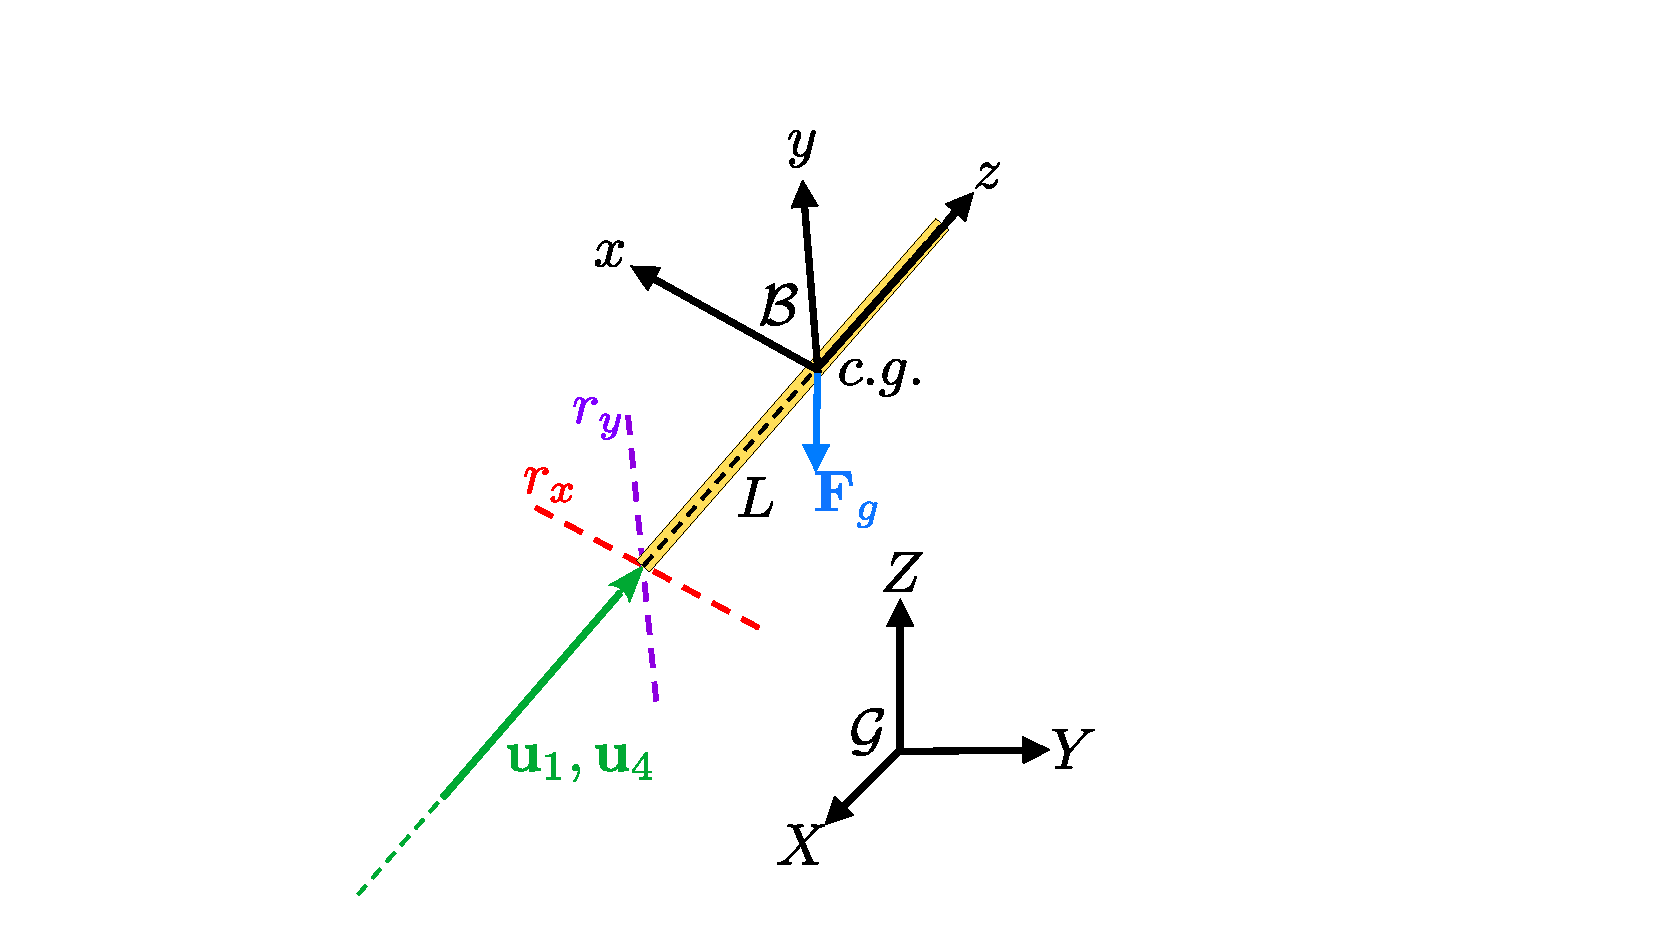
\includegraphics[width = \linewidth]{rdyyy_1.pdf}
    \end{minipage} \\
    \begin{minipage}{0.3\linewidth}
        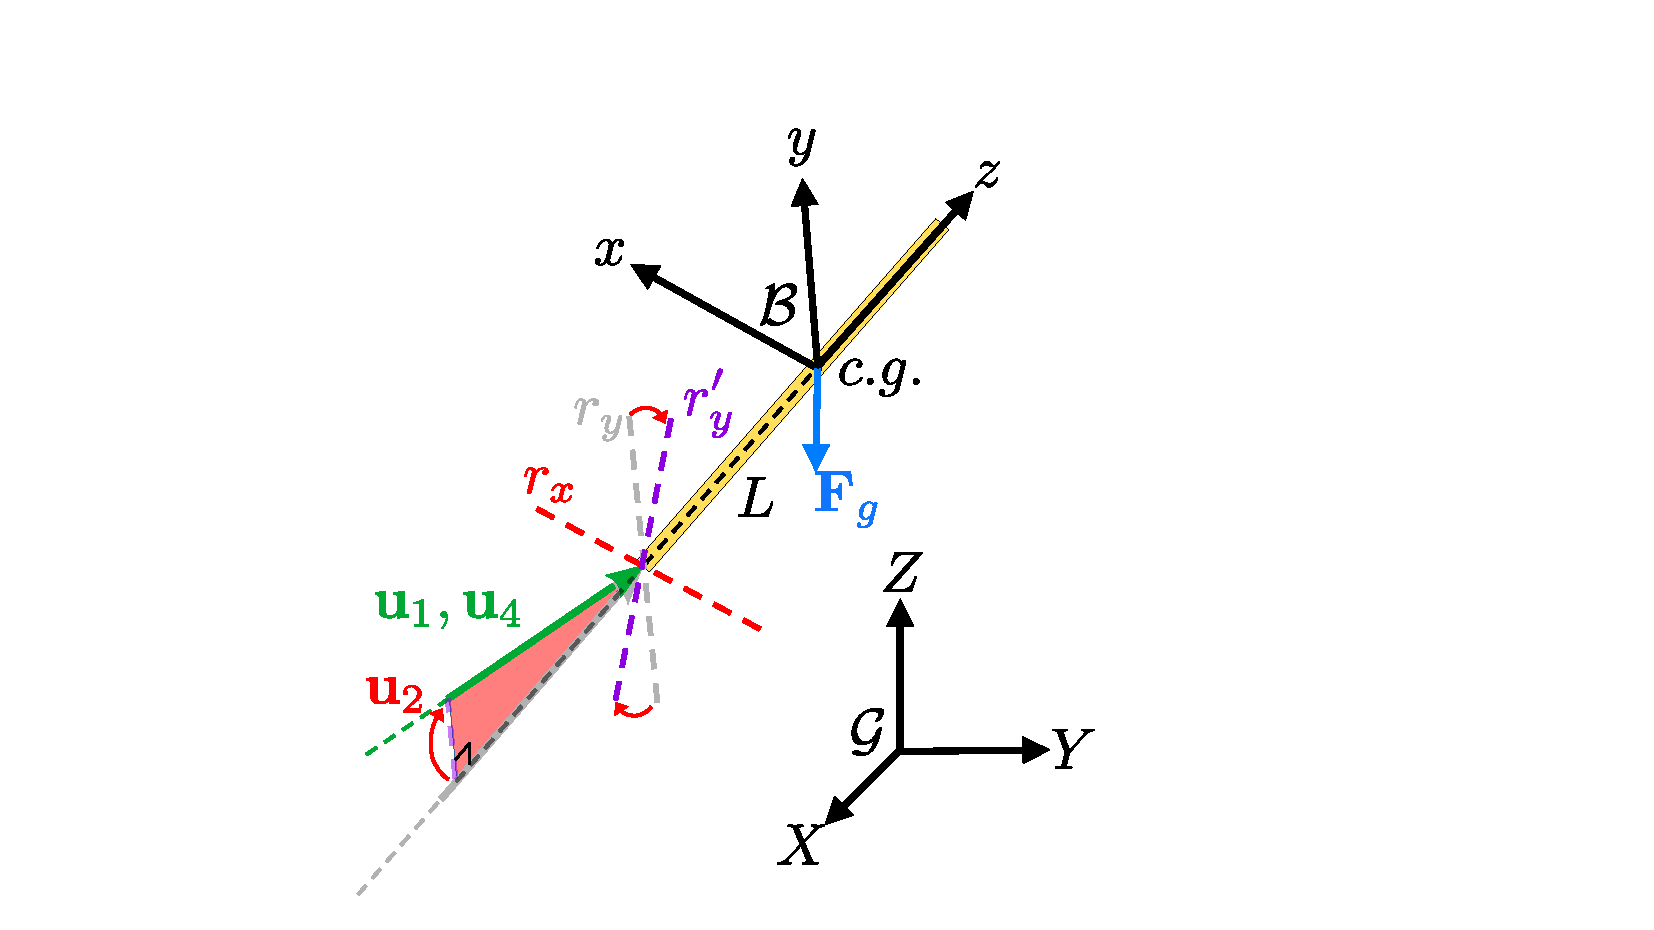
\includegraphics[width = \linewidth]{rdyyy_2.pdf}
    \end{minipage}
    \begin{minipage}{0.3\linewidth}
        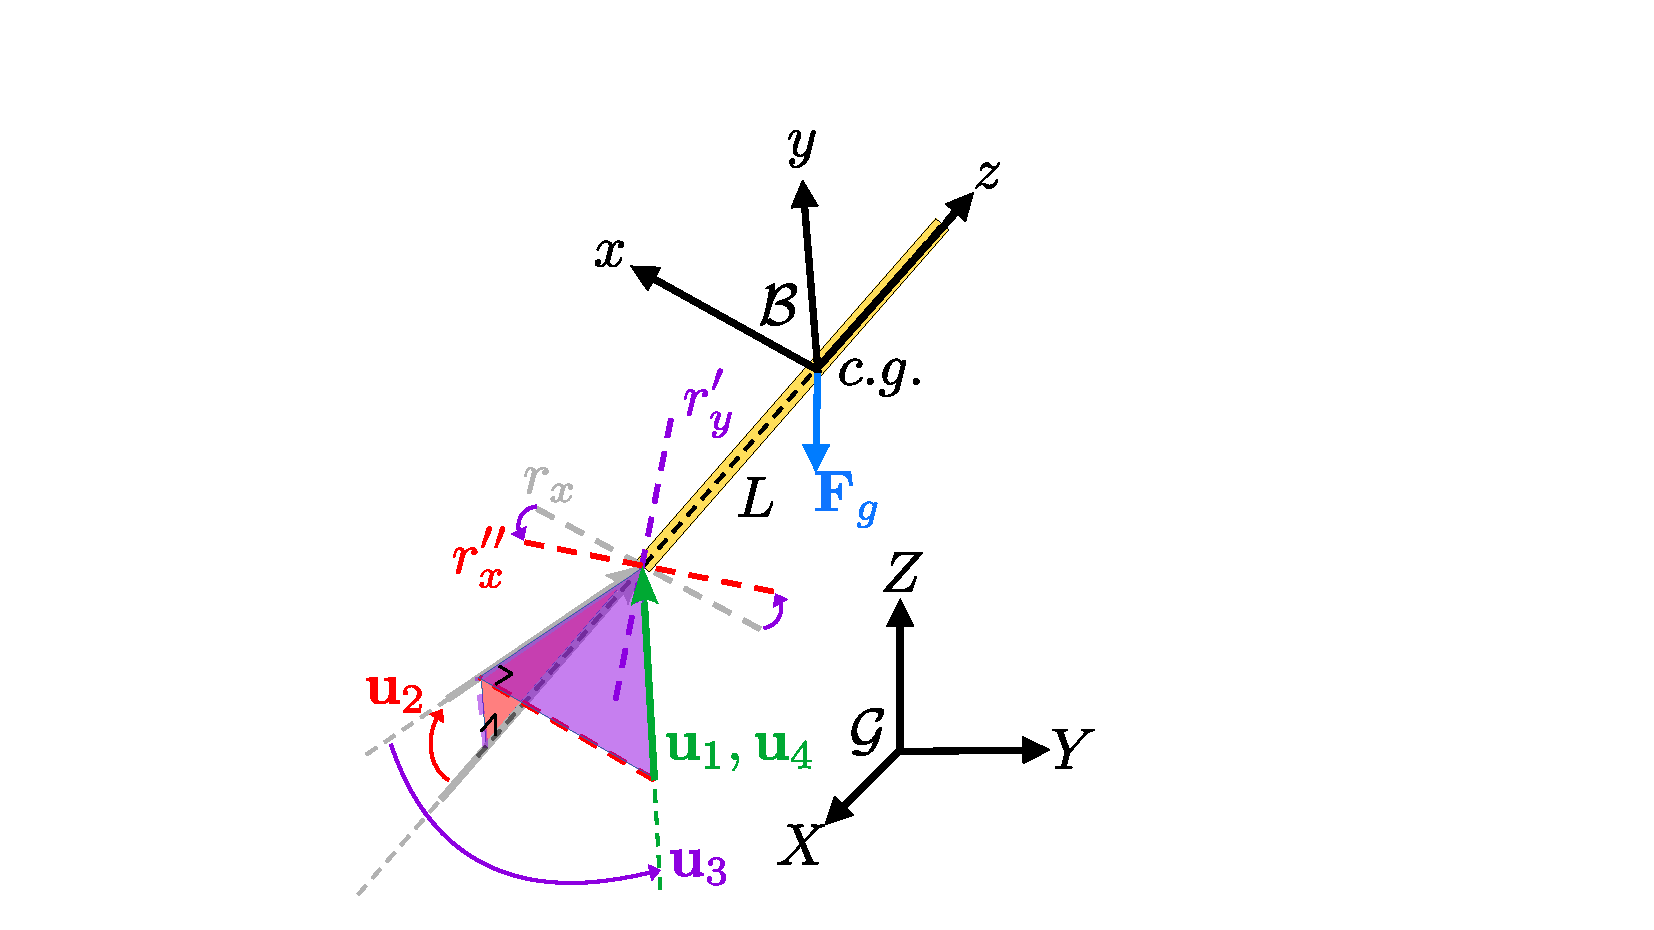
\includegraphics[width = \linewidth]{rdyyy_3.pdf}
    \end{minipage}
    \caption{Illustration of the rocket-type UAV force analysis.}
    \label{fig:6Dof_Rocket_Dynamics2}
\end{figure}


\section{Table Example}



\begin{table}[ht]
    \centering
    \caption{Simulated system parameters}
    \begin{tabular}{ccccc}
        \toprule
        $m$ (kg) & $g$ (m/s${}^2$) & $\bmrm{J}$ (kg-m${}^2$) & $L$ (m) & $C_d$ \\
        \midrule
        & \\
        $0.65$ & $9.8$ & $\begin{bmatrix}
        0.1287 & 0 & 0 \\
        0 & 0.1287 & 0 \\
        0 & 0 & 0.052
        \end{bmatrix}$ & $0.45$ & $0.05$ \\ & \\
        \bottomrule
    \end{tabular}
    \label{tab:Sim_Para}
\end{table}

\begin{table}[H]
    \setlength{\abovecaptionskip}{0cm}
    \caption{Levenberg-Marquardt Method pseudo code.}
        \begin{minipage}{\linewidth}
            \begin{algorithm}[H]
                \caption{Levenberg-Marquardt Method}\label{alg:LM}
                \begin{algorithmic}
                    \State \textbf{given} an initial value $\bmrm{u}^{(0)}$, $\lambda^{(0)} = 1000$, $\epsilon = 10^{-5}$.
                    \Repeat
                    \State 1.~Determine a Jacobian matrix $\bmrm{J}_{\bmrm{r}}^{(k)}$.
                    \State 2. Update the damping parameter $\lambda^{(k)}$.
                    \State 3.~Update the LM step. 
                    \State ~~~~$\bmrm{d}^{(k)} = -\left({\bmrm{J}_{\bmrm{r}}^{(k)T}} \bmrm{J}_{\bmrm{r}}^{(k)} +\lambda^{(k)} {\bmrm{I}_4} \right)^{-1} \bmrm{J}_{\bmrm{r}}^{(k)T} \bmrm{r}(\bmrm{u}^{(k)})$.
                    \State 4.~Update the control variables.
                    \State ~~~~$\bmrm{u}^{(k+1)} = \bmrm{u}^{(k)} +\bmrm{d}^{(k)}$.
                    \State ~~~~$k \leftarrow k+1$.
                    \State 5. Compute the residual error vector to evaluate the stopping condition.
                    \State ~~~~$\bmrm{r}(\bmrm{u}^{(k+1)}) = [r_1, r_2, r_3, r_4]^T$ 
                    \Until{$\| \bmrm{r} \| < \epsilon $ is satisfied, $\vec{u}^{*}=\vec{u}^{(k+1)}$.}
                \end{algorithmic}
            \end{algorithm}
        \end{minipage}
    \end{table}

\section{Subfiles Example}

\subfile{Subfolder_example/sec_subfiles.tex}

\appendix

\section{Matlab Code}
\begin{lstinputlisting}[style=Matlab]{main.m}
\end{lstinputlisting}

\section{C++ Code}
\begin{lstinputlisting}[style=C++]{main.cpp}
\end{lstinputlisting}

\end{document}